\documentclass[10pt]{article}
\usepackage{tikz}
\usetikzlibrary{shapes.misc}
\usepackage[margin=0cm]{geometry}
\pagestyle{empty}
\tikzstyle{every node}=[cross out, draw, red]

\begin{document}

\vspace*{\fill}
\begin{center}
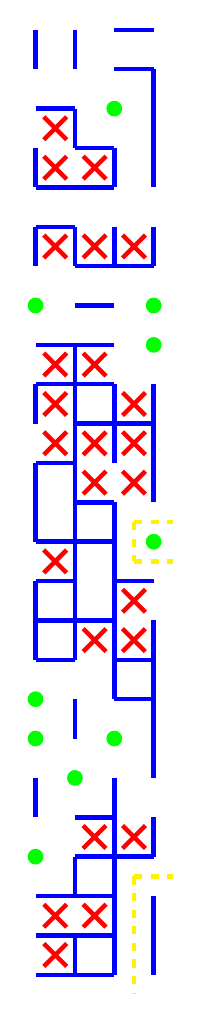
\begin{tikzpicture}[x=0.5cm, y=-0.5cm, ultra thick, blue]
% Walls
    \draw (2,0) -- (3,0);
    \draw (2,1) -- (3,1);
    \draw (0,2) -- (1,2);
    \draw (1,3) -- (2,3);
    \draw (0,4) -- (2,4);
    \draw (0,5) -- (1,5);
    \draw (1,6) -- (3,6);
    \draw (1,7) -- (2,7);
    \draw (0,8) -- (2,8);
    \draw (0,9) -- (2,9);
    \draw (1,10) -- (3,10);
    \draw (0,11) -- (1,11);
    \draw (1,12) -- (2,12);
    \draw (0,13) -- (2,13);
    \draw (0,14) -- (1,14);
    \draw (2,14) -- (3,14);
    \draw (0,15) -- (2,15);
    \draw (0,16) -- (1,16);
    \draw (2,16) -- (3,16);
    \draw (2,17) -- (3,17);
    \draw (1,20) -- (2,20);
    \draw (1,21) -- (3,21);
    \draw (0,22) -- (2,22);
    \draw (0,23) -- (2,23);
    \draw (0,24) -- (2,24);
    \draw (0,0) -- (0,1);
    \draw (0,3) -- (0,4);
    \draw (0,5) -- (0,6);
    \draw (0,9) -- (0,10);
    \draw (0,11) -- (0,13);
    \draw (0,14) -- (0,16);
    \draw (0,19) -- (0,20);
    \draw (1,0) -- (1,1);
    \draw (1,2) -- (1,3);
    \draw (1,5) -- (1,6);
    \draw (1,8) -- (1,16);
    \draw (1,17) -- (1,18);
    \draw (1,21) -- (1,22);
    \draw (1,23) -- (1,24);
    \draw (2,3) -- (2,4);
    \draw (2,5) -- (2,6);
    \draw (2,9) -- (2,11);
    \draw (2,12) -- (2,17);
    \draw (2,19) -- (2,24);
    \draw (3,1) -- (3,4);
    \draw (3,5) -- (3,6);
    \draw (3,9) -- (3,12);
    \draw (3,15) -- (3,19);
    \draw (3,20) -- (3,21);
    \draw (3,22) -- (3,24);
% Pillars
    \fill[green] (2,2) circle(0.2);
    \fill[green] (0,7) circle(0.2);
    \fill[green] (3,7) circle(0.2);
    \fill[green] (3,8) circle(0.2);
    \fill[green] (3,13) circle(0.2);
    \fill[green] (0,17) circle(0.2);
    \fill[green] (0,18) circle(0.2);
    \fill[green] (2,18) circle(0.2);
    \fill[green] (1,19) circle(0.2);
    \fill[green] (0,21) circle(0.2);
% Inner points in accessible cul-de-sacs
    \node at (0.5,2.5) {};
    \node at (0.5,3.5) {};
    \node at (1.5,3.5) {};
    \node at (0.5,5.5) {};
    \node at (1.5,5.5) {};
    \node at (2.5,5.5) {};
    \node at (0.5,8.5) {};
    \node at (1.5,8.5) {};
    \node at (0.5,9.5) {};
    \node at (2.5,9.5) {};
    \node at (0.5,10.5) {};
    \node at (1.5,10.5) {};
    \node at (2.5,10.5) {};
    \node at (1.5,11.5) {};
    \node at (2.5,11.5) {};
    \node at (0.5,13.5) {};
    \node at (2.5,14.5) {};
    \node at (1.5,15.5) {};
    \node at (2.5,15.5) {};
    \node at (1.5,20.5) {};
    \node at (2.5,20.5) {};
    \node at (0.5,22.5) {};
    \node at (1.5,22.5) {};
    \node at (0.5,23.5) {};
% Entry-exit paths without intersections
    \draw[dashed, yellow] (2.5,12.5) -- (3.5,12.5);
    \draw[dashed, yellow] (2.5,13.5) -- (3.5,13.5);
    \draw[dashed, yellow] (2.5,21.5) -- (3.5,21.5);
    \draw[dashed, yellow] (2.5,12.5) -- (2.5,13.5);
    \draw[dashed, yellow] (2.5,21.5) -- (2.5,24.5);
\end{tikzpicture}
\end{center}
\vspace*{\fill}

\end{document}
